\documentclass[a4paper,parskip]{scrartcl}
\usepackage[usenames,dvipsnames,svgnames,table]{xcolor}
\usepackage[utf8]{inputenc}
\usepackage[ngerman]{babel}
\usepackage{amsmath}
\usepackage{enumerate}
\usepackage{textcomp}
\usepackage{fancyhdr}
\usepackage[a4paper]{geometry}
\usepackage{amsthm}
\usepackage{amsfonts}
\usepackage[version=3]{mhchem}
\usepackage{graphicx}
\usepackage{subfig}
\usepackage{float}

\bibliographystyle{apalike}


\author{Sven Jandura \& Edward Wang} 
\title{Auswertung des Versuchs H2}

\geometry {
  top=0.75in,
  headsep=3ex,
  bottom=0.75in,
}

\fancypagestyle{plain}{
  \fancyhf{}
  \fancyhead[L]{Sven Jandura \& Edward Wang}
  %\fancyhead[C]{} %Center
  \fancyhead[R]{Seite \thepage}
}

\renewcommand{\headrule}{\color{Black}\hrule height\headrulewidth\hfill}
\pagestyle{plain}

\let\stdsection\section\renewcommand\section{\newpage\stdsection}

\newtheorem{mydef}{Definition}
\newtheorem{mythe}{Satz}


\begin{document}

\maketitle

\tableofcontents

\section{Grundlagen}

In der Quantenmechanik werden die Elektronenorbitale von Atomen durch diskrete Energieniveaus beschrieben. Dabei kann es zu Übergänge zwischen diesen Zuständen kommen, bei denen ein Photon absorbiert bzw. emittiert wird. Die Frequenz dieses Photons wird dann gemäß der Planck-Formel durch $E_2 - E_1 = h \nu$ gegeben. Durch Messung dieser Resonanzfrequenz $\nu$ kann man die Abstände der Energieniveaus bestimmen. Allerdings lässt sich diese Spektrallinie nicht beliebig scharf messen, sondern sie besitzt eine gewisse Linienbreite. Grund dafür sind, u.a., die Stoßverbreiterung, die durch Wechselwirkungen zwischen verschiedenen Atomen verursacht wird, die Dopplerverbreiterung und die natürliche Linienbreite. Die natürliche Linienbreite kommt dadurch zustande, dass diese angeregte Zustände nur kurzlebig sind, und wegen der Energie-Zeit-Unschärfe ist die Energie dieses angeregten Zustandes also nicht genau definiert. Die Linie nimmt die Form eines Lorentz-Peaks:
\begin{equation*}
    I(\omega) = I_0 \frac{1}{\pi} \frac{\gamma/2}{(\omega - \omega_0)^2 + (\gamma / 2)^2}
\end{equation*}
Die Doppler-Verbreiterung entsteht wegen der statistischen Geschwindigkeitsverteilung der Teilchen im Gas. Dadurch kommt es zu einer Doppler-Verschiebung des Lichts, gemäß
\begin{equation*}
    \omega' = \omega_0 \left(1 - \frac{v_z}{c} \right)
\end{equation*}
Somit berechnet sich die absorbierte Intensität zu einem Gauß-Peak:
\begin{equation*}
    I(\omega) = I(\omega_0) e^{- \left( \frac{\omega - \omega_0}{\delta \omega_D/\sqrt{4 ln 2}} \right)^2}
\end{equation*}
wobei
\begin{equation*}
    \delta \omega_D = \frac{\omega_0}{c} \sqrt{\frac{8 kT ln2}{m}}
\end{equation*}

Das Rubidium-Atom besitzt nur ein Valenzelektron, d. h., die inneren Schalen sind abgeschlossen und tragen nicht für den Gesamtdrehimpuls bzw. Spin bei. Außerdem kann man die Wechselwirkungen zwischen dieses Valenzelektron und die restlichen vernachlässigen, weshalb es als wasserstoffähnlich bezeichnet wird. Wir betrachten die beiden Isotope Rb-85 und Rb-87, die stabil sind, und dessen Kernspins jeweils $5/2$ bzw. $3/2$ beträgt. Wir berücksichtigen zum einen die Grobstruktur, die durch den Abstand der Elektronen zum Kern ensteht, die Feinstruktur, in der die Spin-Bahn-Kopplung berücksichtigt wird, d.h. die Wechselwirkung zwischen den von dem Spin und dem Bahndrehimpuls erzeugten magnetischen Momenten, und die Hyperfeinstruktur, bei der die Kopplung zwischen den Gesamtdrehimpuls und den Kernspin betrachtet wird.

Somit spaltet sich die D2-Linie, die durch den Übergang zwischen den $5^2s_{1/2}$ und den $5^2p_{3/2}$ Zuständen erzeugt wird, in 6 Linien auf.

\section{Versuchsdurchführung}

\subsection{Absorptionsspektroskopie}

 Bei der Absorptionsspektroskopie messen wir das transmittierte Licht durch das Rubidium-Gas. Dabei erwarten wir, dass bei der Durchstimmung der Laserfrequenz eine Senkung der transmittierten Intensität bei den Übergangsfrequenzen beobachtet wird. Das Experiment wurde so aufgebaut, dass ein Laserstrahl durch ein Prismenpaar geschickt wird, damit er rund wird, dann durchquert er ein $\lambda /2$ Plättchen und einen polarisierenden Strahlteiler, die Rubidium-Zelle, und wird schließlich durch eine Linse in die Photodiode fokussiert, wo dann die Intensität des Lichts gemessen wird. Der reflektierte Teil im Strahlteiler wird in einem Referenzresonator der Länge 10cm geleitet, damit der freie Spektralbereich nach 
\begin{equation}
	\Delta \nu = \frac{c}{2d}
	\label{Spektralbereich}
\end{equation}
bestimmt werden kann.
Ein Funktionsgenerator durchstimmt den Laser mit einer Frequenz von ca. 20 Hz und die Intensität wird mit einem Oszilloskop gespeichert.

\subsection{Sättigungsspektroskopie}

Ziel der Sättigungsspektroskopie ist es, die Dopplerverbreiterung zu vermeiden. Dabei ist der Unterschied zur Absorptionsspektroskopie, dass der Strahl die Zelle zweimal in umgekehrten Richtungen durchquert. Experimentell wird es umgesetzt, indem der linear polarisierte Strahl nach der Rubidium-Zelle durch einen ND-Filter abgeschwächt wird, durch ein $\lambda/4$ Plättchen zirkular polarisiert, in einem Spiegel reflektiert und wieder linear polarisiert wird, bevor er die Rubidium-Zelle nochmal durchläuft. Bei der Reflektion wird die zirkulare Polarisation umgedreht, sodass der Teststrahl nach der $\lambda/4$ Platte senkrecht zum Pumpstrahl polarisiert ist, und deshalb beim polarisierenden Strahlteiler komplett in der Diode reflektiert wird. Auch hier wird der Strahl durch eine Linse fokussiert.

Bei diesem Versuch erwarten wir die selben Senkungen zu beobachten, wie in der Absorptionsspektroskopie, allerdings mit sogenannten Lamb-Dips. Wenn der Pumpstrahl die Resonanzfrequenz eines Übergangs trifft, regt er Atome im Gas an, und wenn diese Atome entlang der Verbreitungsachse des Strahls eine Geschwindigkeit nahe Null haben, wird aus Sicht dieser Atome der Teststrahl die selbe Frequenz besitzen wie der Pumpstrahl; allerdings können sie nicht durch den Teststrahl angeregt werden, da diese Anregung schon durch den Pumpstrahl gesättigt wurde. Somit entstehen Peaks im Intensitätsprofil.

\section{Auswertung}

\subsection{Absorbtionsspektrum}

Es werden die Peaks des Referenzresonator gegen die Zeit aufgetragen und mit einem Polynom dritter Ordung gefittet, um die Nichtlinearität der Verstimmung des Lasers zu korrigieren.

\begin{figure}[h]
\centering
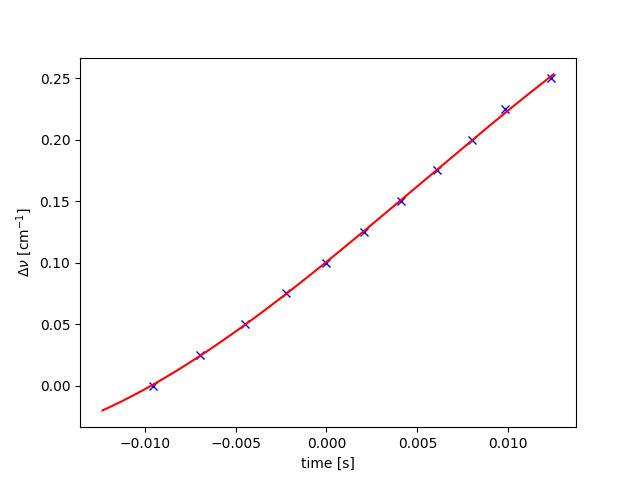
\includegraphics[scale = 0.5]{./absorbtion/frequencyCorrection}
\end{figure}

Die Frequenz des Lasers sei $\nu_0+\nu$, wobei $\nu_0=\frac{c}{780\mathrm{nm}}$ die ungefähre Frequenz des Lasers ist. Es ist $\nu \ll \nu_0$.
Betrachte einen Übergang mit Energiedifferenz $h\nu_1$ und einer Linienform ohne Dopplerverbreiterung $L(\nu)$.  Die Absorbierte Intensität bei Laserfrequenz $\nu$ ist proportional zu

$$\int_{-\infty}^{\infty} dv f_{MB}(v)L(\nu\sqrt{1-v/c}) \approx \int_{-\infty}^{\infty} dv f_{MB}(v)L(\nu_0+\nu-\nu_0 v/(2c))$$

Die Näherung ist gerechtfertigt, da für thermische Geschwindigkeiten $v \ll c$ und weil $\nu \ll \nu_0$. Da $L$ scharf um $\nu_0 + \nu_1$ gepeakt ist, kann man $L$ als Delta-Funktion approximieren. Die absorbierte Intensität ist daher proportional zu

$$f_{MB}(2c(\nu-\nu_1)/\nu_0) \sim e^{-mc^2(\nu-\nu1)^2/(2k_BT\nu_0^2)}$$

Für $N$ Übergänge bei Frequenzen $\nu_0+\nu_1,...,\nu_0+\nu_N$ lautet die Formel für die gemessene Intensität an der Photodiode also

\begin{equation}
I(\nu) = I_0(\nu) - \sum_{n=1}^N I_n e^{-mc^2(\nu-\nu_n)^2/(2k_BT\nu_0^2)}
\label{AbsorbtionFit}
\end{equation}

Da man mit den Messdaten nicht die Übergänge von einem s-Hyperfeinniveau zu verschiedenen p-Hyperfeinniveaus unterscheiden kann, fassen wir alle Übergänge, die vom selben s-Hyperfeinniveau ausgehen, zu einem zusammen. Wir fitten (\ref{AbsorbtionFit}) an die Messdaten. Dabei verwenden wir für $I_0$ ein Polynom zweiter Ordnung.

\begin{figure}[h]
\centering
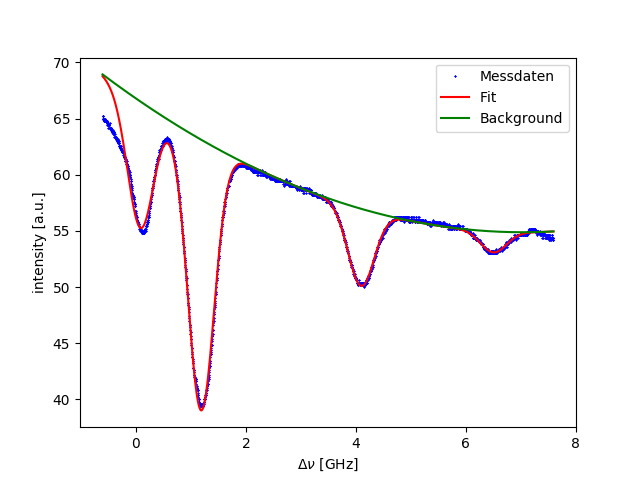
\includegraphics[scale = 0.5]{./absorbtion/fit.png}
\end{figure}

Die Abweichung des Fits an der linken Seite führen wir auf die Nichtlinearität der Durchstimmung des Lasers zurück. Der Fit weicht an der linken Seite nur vor dem ersten Peak des Referenzresonators ab. Unsere Interpolation von oben kann augenscheinlich nicht verwendet werden, um die Frequenz-Zeit Abhängigkeit links des ersten Peaks des Referenzresonators zu extrapolieren. Auch beim Experiment wurde beobachtet, dass der Laser in einem Frequenzbereich annähernd linear durchgestimmt wird, an den Rändern aber sehr nichtlinear.

Wir erhalten folgende Werte:

\begin{align*}
\nu_1 &= 0.082 \pm 0.001 GHz \\
\nu_2 &= 1.1854 \pm 0.0003 GHz \\
\nu_3 &= 4.094 \pm 0.002 GHz\\
\nu_4 &= 6.501 \pm 0.005 GHz \\
T&=350 \pm 2 K
\end{align*}

Damit ergeben sich die Abstände im Termschema zu $1.103 \pm 0.002 GHz$,  $2.909 \pm 0.003 GHz$ und $6.419 \pm 0.006 GHz$. Die Abweichungen zu den Literaturwerten können zum Teil damit erklärt werden, dass wir die Übergänge zu unterschiedlichen p-Hyperfeinniveaus in dem Verfahren nicht auflösen konnten, und deshalb mit einer einzigen Gauß-Funktion gefittet haben. Da diese Kurve in der Tat die Summe dreier Kurven mit unterschiedlichen Frequenzen und Intensitäten ist, kann man diese Abstände nicht genau bestimmen. Außerdem kennen wir die Abstände zwichen den p-Niveaus im Rb-85 und im Rb-87 nicht.

\subsection{Sättigungsspektroskopie}

Betrachten wir die Übergänge wie oben. Der vom Pumpstrahl mit Frequenz $\nu_0+\nu$ angeregte Anteil der Atome mit Geschwindigkeit $v$ beträgt

$$n(\nu, v) = \sum_{i=1}^N A_i L_i(\nu_0+\nu-\nu_0 v/(2c))$$

mit Konstanten $A_1, ..., A_N$. Die gemessene Intensität beträgt dann

$$I(\nu) = I_0(\nu)-\int_{-\infty}^{\infty} f_{MB}(v)(1-n(\nu, v))\sum_{j=1}^N B_j L_i(\nu_0+\nu+\nu_0 v/(2c))$$

Mit Konstanten $B_1, ..., B_N$ und Ausgangsintensität $I_0(\nu)$. Der erste Summand im Integraten ist der selbe Term wie bei der Absorbtionsspektroskopie. Den zweiten Term nähern wir, indem wir ausnutzen, dass  $L_i(\nu_0+\nu-\nu_0 v/(2c)) L_j(\nu_0+\nu+\nu_0 v/(2c))$ nur für $v \approx 2c \frac{\nu_i-\nu}{\nu_0}$ nicht verschwindend ist. Deshalb können wir $f_{MB}(v)$ als konstant annehmen und haben nur noch den Term

$$T_{ij}=\int_{-\infty}^\infty dv L_i(\nu_0+\nu-\nu_0 v/(2c)) L_j(\nu_0+\nu+\nu_0 v/(2c))$$

Sei $L_\gamma$ die Lorenzverteilung um 0 mit FWHM $\gamma$. Wir nehmen $L_i(x) = L_{\gamma_i}(x-(\nu_0+\nu_i)$ and. Dann ist

\begin{align*}
T_{ij} &= \frac{2c}{\nu_0}\int_{-\infty}^\infty du L_{\gamma_i}(2\nu-(\nu_i+\nu_j)-u)L_{\gamma_j}(u)\\
&= \frac{2c}{\nu_0} (L_{\gamma_i} * L_{\gamma_j})(2\nu-(\nu_i+\nu_j)) \\
&= \frac{2c}{\nu_0} L_{\gamma_i+\gamma_j}(2\nu-(\nu_i+\nu_j)) \\
\end{align*}

Damit ergibt sich insgesamt eine Fitfunktion
\begin{equation}
I(\nu) = I_0(\nu)-\sum_{i=1}^N B_i e^{-mc^2(\nu-\nu_i)^2/(2k_BT\nu_0^2)} +\sum_{\substack{i,j=1\\i\leq j}}^N C_{ij} L_{\gamma_i+\gamma_j}(2\nu-(\nu_i+\nu_j))
\label{SaettigungsFit1}
\end{equation}


mit Konstanten $C_{ij}$. Wir haben $T_{ij}=T_{ji}$ ausgenutzt.\\

Wir haben jeden der vier großen Peaks individuell gefittet. Ein Fit mit der Funktion aus (\ref{SaettigungsFit1}) war jedoch leider nicht möglich, der Fit ist nicht konvergent. Wir führen das darauf zurück, dass die Variation der $B_i$ die Funktion kaum verändert, solange ihre Summe konstant bleibt. Stattdessen haben wir, wie bei der Absorbtionsspektroskopie, die Gausspeaks zu einem einzelnen zusammengefasst und mit der Funktion

 \begin{equation}
I(\nu) = I_0(\nu)-B e^{-mc^2(\nu-\nu_{Gauss})^2/(2k_BT\nu_0^2)} +\sum_{\substack{i,j=1\\i\leq j}}^N C_{ij} L_{\gamma_i+\gamma_j}(2\nu-(\nu_i+\nu_j))
\label{SaettigungsFit2}
\end{equation}

gefittet. $I_0$ haben wir als Polynom ersten Grades gefittet. Die weiteren Fit Parameter sind $B$, $\nu_{Gauss}$, $T$, $C_{ij}$ und $\gamma_i$. Das Ergebnis der Fits mit und ohne Dopplerhintergrund ist in Abbildung~\ref{fig:Abbildung1} dargestellt.

\begin{figure}[p]
\centering
\begin{tabular}{cc}
    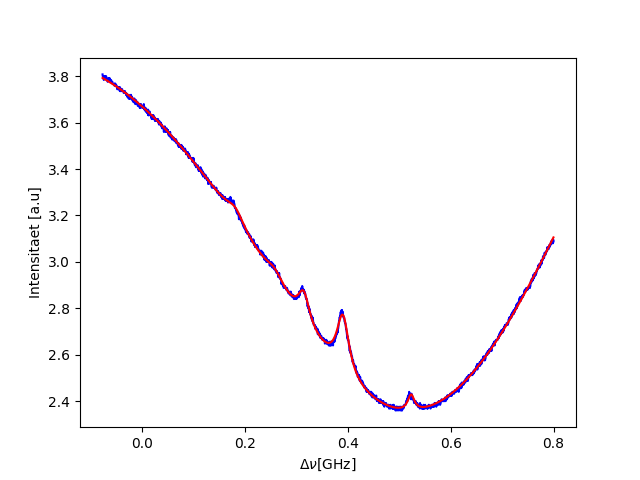
\includegraphics[scale = 0.45]{./saturation/peak1/fit.png}  &  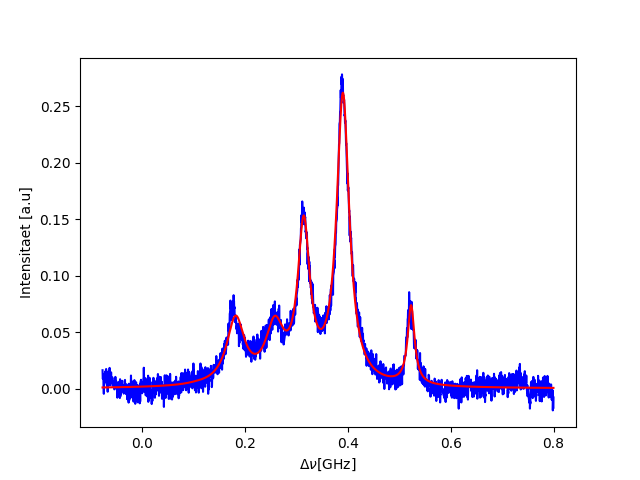
\includegraphics[scale = 0.45]{./saturation/peak1/gaussCorrected.png}  \\
    {\footnotesize Peak 1} & {\footnotesize Peak 1 ohne Dopplerhintergrund}  \\
    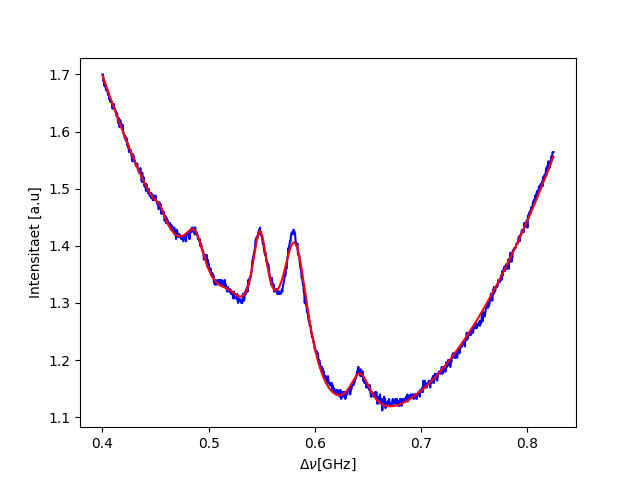
\includegraphics[scale = 0.45]{./saturation/peak2/fit.png}  &  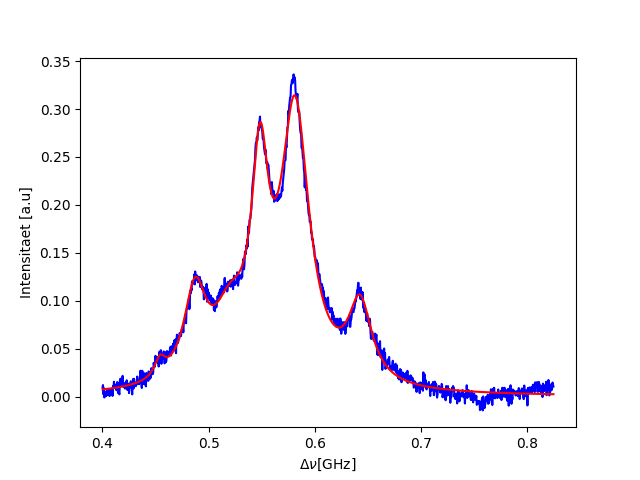
\includegraphics[scale = 0.45]{./saturation/peak2/gaussCorrected.png}  \\
    {\footnotesize Peak 2} & {\footnotesize Peak 2 ohne Dopplerhintergrund}  \\
    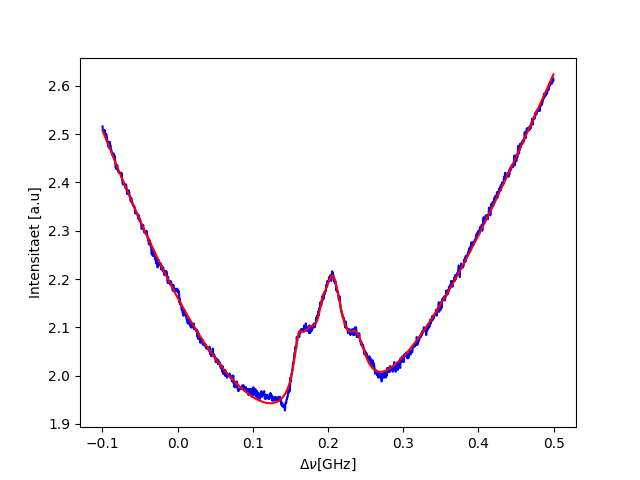
\includegraphics[scale = 0.45]{./saturation/peak3/fit.png}  &  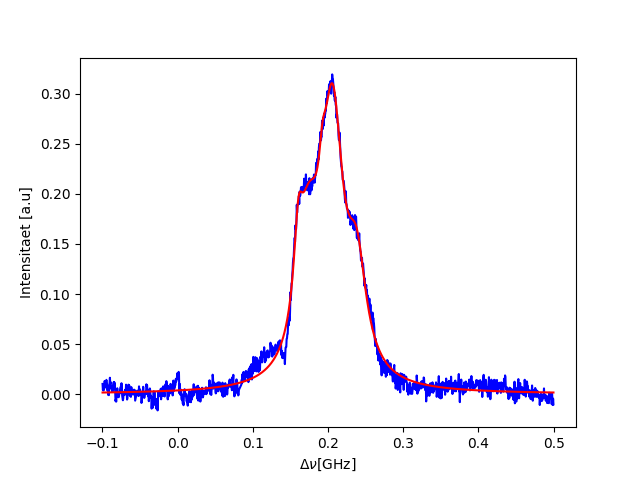
\includegraphics[scale = 0.45]{./saturation/peak3/gaussCorrected.png}  \\
    {\footnotesize Peak 3} & {\footnotesize Peak 3 ohne Dopplerhintergrund}  \\
    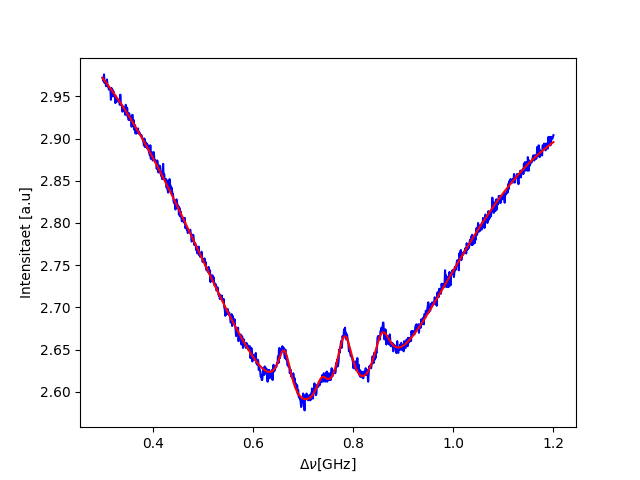
\includegraphics[scale = 0.45]{./saturation/peak4/fit.png}  &  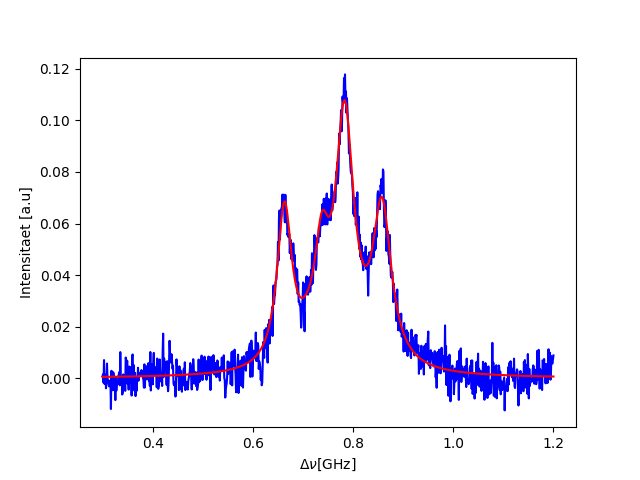
\includegraphics[scale = 0.45]{./saturation/peak4/gaussCorrected.png}  \\
    {\footnotesize Peak 4} &  {\footnotesize Peak 4 ohne Dopplerhintergrund}  \\
\end{tabular}
\caption{Fits}
\label{fig:Abbildung1}
\end{figure}

Wir erhalten folgende Frequenzen:

Übergänge von Rb 87 von $F=2$:

\begin{align*}
\nu_{F'=1} &= 105.7 \pm 0.4 MHz \\
\nu_{F'=2} &= 257.9 \pm 0.3 MHz \\
\nu_{F'=3} &= 523.1 \pm 0.2 MHz  
\end{align*}

Übergänge von Rb 85 von $F=3$:

\begin{align*}
\nu_{F'=2} &= 454.2 \pm 0.3 MHz \\
\nu_{F'=3} &= 520.6 \pm 0.3 MHz \\
\nu_{F'=4} &= 642.7 \pm 0.2 MHz  
\end{align*}

Übergänge von Rb 85 von $F=2$:

\begin{align*}
\nu_{F'=1} &= 147.0 \pm 0.5 MHz \\
\nu_{F'=2} &= 174.1 \pm 0.5 MHz \\
\nu_{F'=3} &= 238.2 \pm 0.3 MHz  
\end{align*}

Übergänge von Rb 87 von $F=1$:

\begin{align*}
\nu_{F'=0} &= 617.4 \pm 0.8 MHz \\
\nu_{F'=1} &= 708.6 \pm 0.7 MHz \\
\nu_{F'=2} &= 857.8 \pm 0.5 MHz  
\end{align*}

Damit ergeben sich die Differenzen zwischen den Niveaus zu $28 \pm 1 MHz$, $66.4 \pm 0.6MHz$ bzw. $64.1 \pm 0.8 MHz$ und $122.1 \pm 0.5 MHz$ für Rb 85 sowie $91 \pm 2 MHz$, $152.2 \pm 0.7 MHz$ bzw. $149 \pm 2 MHz$ und  $265.2 \pm 0.5 MHz$ für Rb 87.\\

Man  kann nun noch versuchen, die Abstände der s-Hyperfeinniveaus beider Isotope genauer zu bestimmen, indem man mit $\nu_{Gauss} - \nu_i$ korrigiert, d.h., man betrachtet Übergänge zu den einzelnen p-Hyperfeinniveaus und berechnet daraus die Differenz. In Rb-85 ist das für die p-Niveaus mit $F=2$ und $F=3$, möglich, in Rb-87 fur $F=1$ und $F=2$. Man erhält
$3.07 \pm 0.01 GHz$ bzw $3.10 \pm 0.02 GHz$ für Rb-85 und $6.51 \pm 0.01 GHz$ bzw $6.68 \pm 0.02 GHz$.

Unsere gemessene Werte für die p-Hyperfeinniveaus im Vergleich zu den Literaturwerten (\cite{Ref:1}, \cite{Ref:2}) sind in Abbildung \ref{fig:Abbildung2} dargestellt.

\begin{figure}[h]
\centering
\begin{tabular}{cc}
    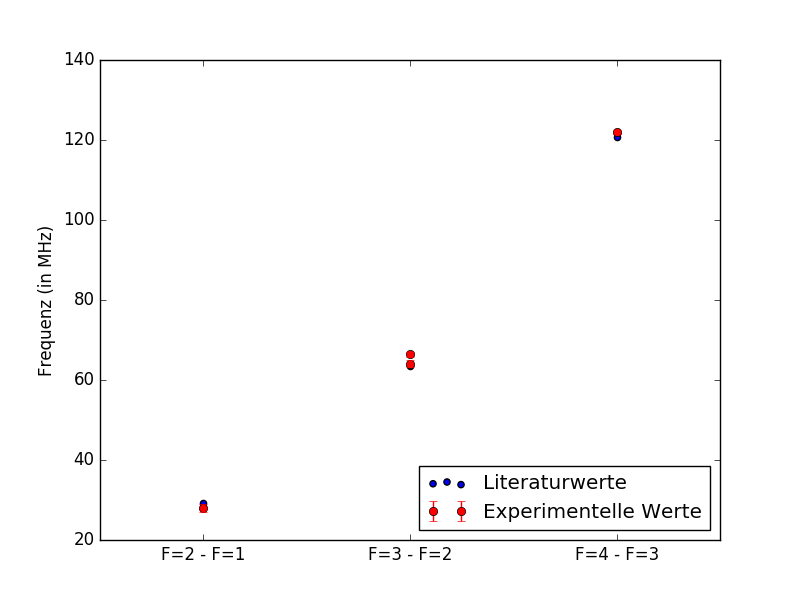
\includegraphics[width = 0.5\textwidth]{daten_Rb-85.png}  &  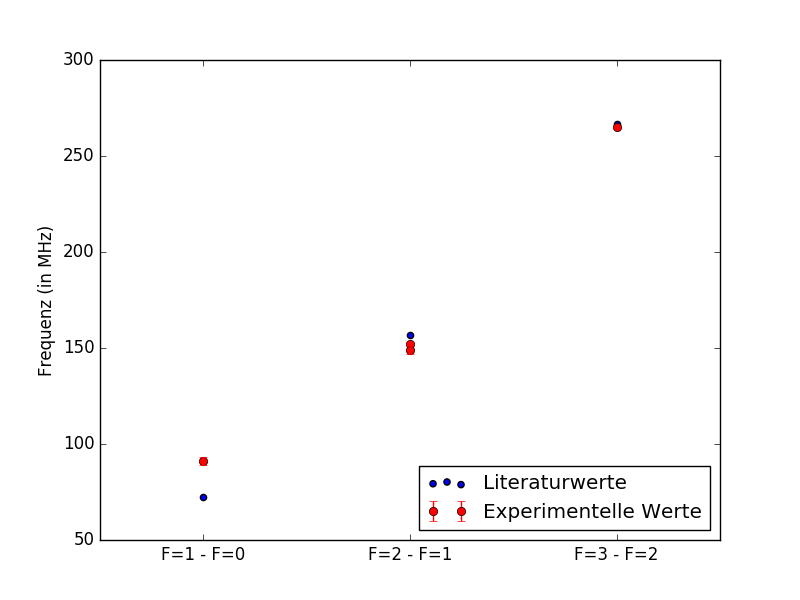
\includegraphics[width = 0.5\textwidth]{daten_Rb-87.png}  \\
    {\footnotesize Rb-85} & {\footnotesize Rb-87}  \\
\end{tabular}
\caption{Werte im Vergleich}
\label{fig:Abbildung2}
\end{figure}

\subsection{Fehlerdiskussion}

Die beobachtete natürliche Linienbreite der Lamb-Dips ist kein Messfehler, denn es handelt sich um eine intrinsische Unschärfe, wie schon oben beschrieben.

Die Durchstimmung des Lasers ist nicht linear, wir haben sie durch einen Polynom 3. Grades gefittet. Bei der Betrachtung der einzelnen Peaks bei der Sättigungsspektroskopie hatten wir jeweils nur zwei Werte aus den Referenzresonator zur Verfügung, sodass wir die Durchstimmung des Lasers als linear annähern mussten. Man hätte diese Durchstimmung korrigieren können, dafür bräuchte man aber das Signal vom Referenzresonator und man müsste die Lasereinstellung fest lassen. In unserem Versuch mussten wir die Einstellungen vom Laser gelegentlich ändern, um ein schärferes Bild der einzelnen Peaks in der Sättigungsspektroskopie zu bekommen.

Die hohe Temperatur des Gases ($350K$) im Vergleich zur Raumtemperatur kann dadurch erklärt werden, dass das Gas vom Laser erhitzt wird. Dieser Effekt ist umso größer, je niedriger der Druck ist.

Man beobachtet, dass die ermittelten Werte zwar nah an den Literaturwerten liegen, aber nicht immer kompatibel sind. In der Tat können wir erwarten, dass unsere Messunsicherheiten größer als die vom Fit ergebenen Werten sind, aufgrund der Schwankungen der verwendeten Geräte, wie die schon besprochene Durchstimmung des Lasers. Da wir sowohl positive als auch negative Abweichungen beobachten, ist es unwahrscheinlich, dass ein systematischer Fehler vorliegt.

Eine größere Abweichung ist im Wert der Energiedifferenz zwischen den p-Hyperfeinniveaus $F=0$ und $F=1$ bei Rb 87 zu erkennen. Ein möglicher Grund dafür ist die Tatsache, dass der mittlere Peak unscharf und unsymmetrsich ist, wie es im letzten Plot der Abbildung \ref{fig:Abbildung1} zu sehen ist. Daher ist die Resonanzfrequenz nicht genau zu ermitteln.

\newpage

\bibliography{reference}

\end{document}

